%auto-ignore
\documentclass[tikz]{standalone}

\usetikzlibrary{automata,positioning,calc}

\begin{document}
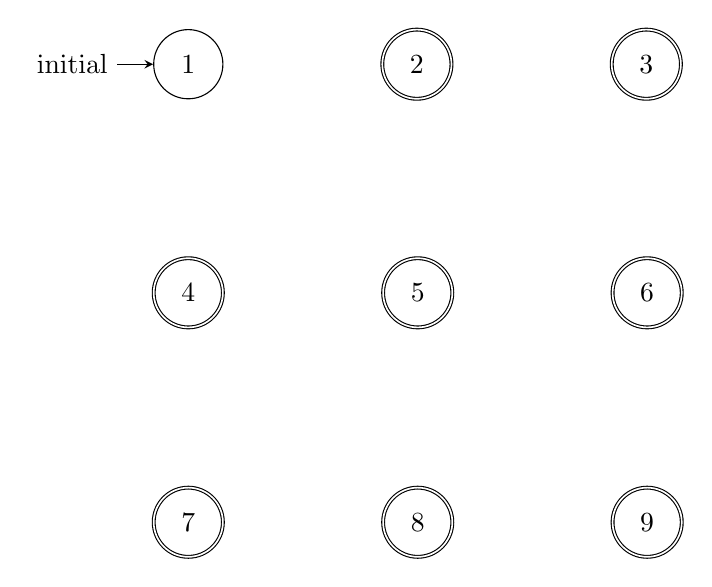
\begin{tikzpicture}[>=stealth,node distance=2,initial text={initial}]

\node [state,initial]   (a00)                {1};
\node [state,accepting] (a10) [right=of a00] {2};
\node [state,accepting] (a20) [right=of a10] {3};

\node [state,accepting] (a01) [below=of a00] {4};
\node [state,accepting] (a11) [right=of a01] {5};
\node [state,accepting] (a21) [right=of a11] {6};

\node [state,accepting] (a02) [below=of a01] {7};
\node [state,accepting] (a12) [right=of a02] {8};
\node [state,accepting] (a22) [right=of a12] {9};

\end{tikzpicture}
\end{document}
